\documentclass{article}
\usepackage{tikz}
\usetikzlibrary{positioning}
\usepackage{pgfplots}
\usepackage{geometry}
\usepackage{amsmath}
\usepackage{amssymb}

%Defining the page dimensions of the latex document
 \geometry{
 a4paper,
 total={170mm,257mm},
 left=20mm,
 top=20mm,
 }



\title{Generalized Hyperplane Tree implementation - aka. GH Tree}


\begin{document}

\textbf{3a. Solution}

Following are the three properties for the Metric Space Indexing that the distance function d must fulfill:
 \begin{itemize}
     \item Symmetry : \[d(a,b) = d(b,a) \]
     \item Non-Negativity : \[d(a,b) \ge 0 , d(a,b) = 0, iff a = b\]
     \item Triangle Inequality : \[d(a,c) \leq d(a,b) + d(b,c) \]
 \end{itemize}
    \begin{enumerate}

   \item\label{l1} 
   For two vectors (or points) $a=(x_a, y_a)$ and $b=(x_b, y_b)$:

 $d(a, b) \mapsto | x_a - x_b | + | y_a - y_b |$.  

We are given two vectors a,b with values d(a,b). To show the values are symmetric, as per euclidean distance formula 
        \[d(a,b) = \sqrt{(xa-xb)^2 + (ya-yb)^2}\]

        (i) \quad for point a(xa,ya) = \[xa^2 - 2.xa.ya + ya^2 = ya^2 - 2.xa.ya + xa^2 = (ya,xa)^2 = |ya,xa|\]
        (ii) for point b(xb,yb) = \[xb^2 - 2.xb.yb + yb^2 = yb^2 - 2.xb.yb + xb^2 = (yb,xb)^2 = |yb,xb|\] 
        (iii) The distance d(b,a) would be  $d(b, a) \mapsto | y_b - y_a | + | x_a - x_b |$.

        From (i), (ii) and (iii), we can say that \textbf{d(a,b)= d(b,a)} which satisfies that the distance between the points fulfills the \textbf{symmetric property}.

The second property the distance should fulfill is the non-negativity for which we assume different values of d(a,b) to prove that d(a,b) \geq 0.

      Let us assume\textbf{ a(xa,ya) = (4,2) and b(xb,yb) = (6,8)}, here the values of xa \neq xb ,  ya \neq yb.
      
     (i) So, \[d(a, b) \mapsto | x_a - x_b | + | y_a - y_b |= \sqrt{(4-6)^2 + (2-8)^2 } = \sqrt {4 +12} = 4 \geq 0\]
     
     It should also prove that d(a,b) = 0 for which we assume a=b to prove d(a,b)=0.
    
     Let us assume\textbf{ a(xa,ya) = (2,2)} and \textbf{b(xb,yb) is (2,2)},\textbf{ xa = xb and ya = yb}
    
     (ii) So, \[d(a, b) \mapsto | x_a - x_b | + | y_a - y_b |= \sqrt{(2-2)^2 + (2-2)^2 } = \sqrt {0 +0} = 0\]
    
    From the points (i) and (ii), we see that it describes the \textbf{non-negativity property}.

    For the query point, we are considering c in this example.
    
    The third property of distance to be fulfilled is the Triangle Inequality. Let us consider the points d(a,b) and d(b,c) to prove this

    \[d(a, b) = | x_a - x_b | + | y_a - y_b |\]
    \[d(b, c) = | x_b - x_c | + | y_b - y_c | \]
    
    \[d(a,b) + d(b,c) = | x_a - x_b | + | y_a - y_b | + | x_b - x_c | + | y_b - y_c | \]
    \quad  \[ = | x_a - x_b | + | x_b - x_c | + | y_a - y_b | + | y_b - y_c | \]
    \quad \[= |x_a - x_b + x_b - x_c| + | y_a - y_b + y_b - y_c | \]
    \quad \[=|x_a - x_c| + |y_a - y_c |\]
    \quad \[=d(a,c)\]

    Hence the above steps prove the \textbf{Triangle Inequality property.}
    
    
    
    \item\label{l2} 
    For two vectors (or points) $a=(x_a, y_a)$ and $b=(x_b, y_b)$:
    $d(a, b) \mapsto ( x_a - x_b )^2 + ( y_a - y_b )^2$.

    Le us consider the points a(2,1), b(1,1) and q(1,2), these points fulfill the \textbf{Symmetric}, \textbf{Non Negativity and Triangle Inequality} properties of the distance.

    Consider the values of a(2,1), b(1,1) and query point q(1,2)

    \[d(a, b) \mapsto ( x_a - x_b )^2 + ( y_a - y_b )^2\]
    \quad \[d(a,q) = (2-1)^2 + (1-2)^2 = 2\]
    \quad \[d(b,q) = (1-1)^2 + (2-1)^2 = 1\]
    \quad \[d(a,b) = (2-1)^2 + (1-1)^2 = 1+0 = 1\]
    \textbf{Symmetric:} d(a,b) = d(b,a) = 1 \textbf{True}
    
    \textbf{Non-Negativity:} d(a,b) \geq 0 =  1 \geq 0 \textbf{ True}

   \textbf{ Triangle Inequality:} d(a,q) \leq d(a,b) + d(b,q) = 2 \leq 1+1 \textbf{True}

   Hence this example \textbf{fulfills} \textbf{all the properties} of the distance between the points.

 
      \item\label{l3} 
      For two strings $s_1$ and $s_2$, where $S$ is the set of characters of the string (e.g.: $S(\text{``Codd''}) = \{\text{`C', `o', `d'}\}$):
      $d(s_1, s_2) \mapsto 2* |S(s_1) \cap S(s_2)| \, / \, (|S(s_1)| + |S(s_2)|)$.\\

      Let us consider the given string \textbf{S =\{\text{'Codd'}\}}, the sub-strings that can be derived from S are
      \[\textbf{s1 = \{\text{`C', `o', `d'}\}}\]
      \[\textbf{s2 = \{\text{`o', `d', `d'}\}}\]
      \[\textbf{s2 = \{\text{`C', `d', `d'}\}}\]

      Calculating the d(s1,s2)
      \[d(s_1, s_2) \mapsto 2* |{'C','o','d'} \cap {'o','d','d'}| \, / \, ({'C','o','d'} + {'o','d','d'}) \]
      \quad  \[= 2*|2|/(3+3) = 2/3\]

      Calculating the d(s2,s3) 
      \[d(s_2, s_3) \mapsto 2* |{'o','d','d'} \cap {'C','d','d'}| \, / \, ({'o','o','d'} + {'C','d','d'}) \]
      \quad  \[= 2*|2|/(3+3) = 2/3\]

      Calculating the d(s1,s3)
      \[d(s_2, s_3) \mapsto 2* |{'C','o','d'} \cap {'C','d','d'}| \, / \, ({'C','o','d'} + {'C','d','d'}) \]
      \quad  \[= 2*|2|/(3+3) = 2/3\]

    \textbf{Symmetric:} d(s_1,s_2) = d(s_2,s_1) = 1 \textbf{True}

    \textbf{Non-Negativity:} d(s_1,s_2) \geq 0 =  2/3 \geq 0 \textbf{ True}

   \textbf{Triangle Inequality:} d(s_1,s_3) \leq d(s_1,s_2) + d(s_2,s_3) = 2/3 \leq 2/3+2/3 \textbf{ False}

   Hence the this distance in this example \textbf{doesn't fulfill} the \textbf{Triangle Inequality property.}

    \end{enumerate}
\\

\newpage


\textbf{4a. Solution:}
\\
\\
\\
\textbf{Generalized Hyperplane Tree implementation}
\\
\\
\\
\\
\\
\\
\begin{center}
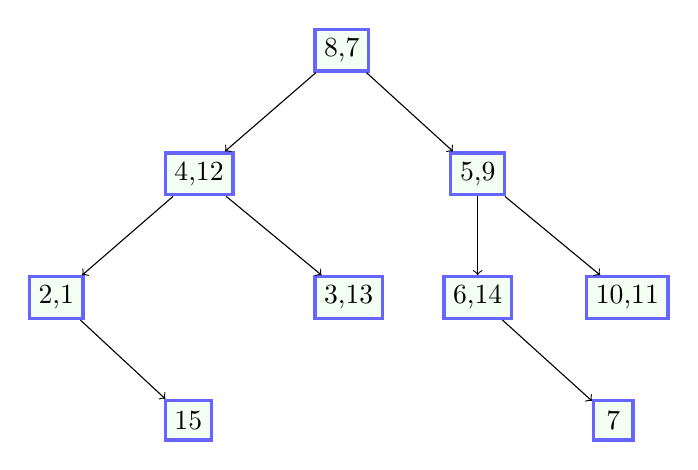
\begin{tikzpicture}
[
squarednode/.style={rectangle, draw=blue!60, fill=green!5, very thick, minimum size=5mm},
]

%\begin{center}
     %Nodes
    \node[squarednode]      (maintopic)                                    {8,7};
    \node[squarednode]      (leftchild)       [below left=of maintopic]    {4,12};
    \node[squarednode]      (rightchild)      [below right=of maintopic]   {5,9};
    \node[squarednode]      (l-leftchild)     [below left = of leftchild]  {2,1};
    \node[squarednode]      (l-rightchild)      [below right = of leftchild] {3,13};
    \node[squarednode]      (r-leftchild)    [below = of rightchild]       {6,14};
    \node[squarednode]       (r-rightchild)   [below right= of rightchild] {10,11};
    \node[squarednode]      (l-l-l)           [below right = of l-leftchild] {15};
    \node[squarednode]      (r-l-r)             [below right = of r-leftchild] {7};
    
    %Lines
    \draw[->] (maintopic) -- (leftchild);
    \draw[->] (maintopic) -- (rightchild);
    \draw[->]   (leftchild) -- (l-leftchild);
    \draw[->]   (leftchild) -- (l-rightchild);
    \draw[->]   (rightchild) -- (r-leftchild);
    \draw[->]   (rightchild) -- (r-rightchild);
    \draw[->]    (l-leftchild) -- (l-l-l);
    \draw[->]   (r-leftchild) -- (r-l-r);
    
\end{tikzpicture}
\end{center}
\\

\begin{center}
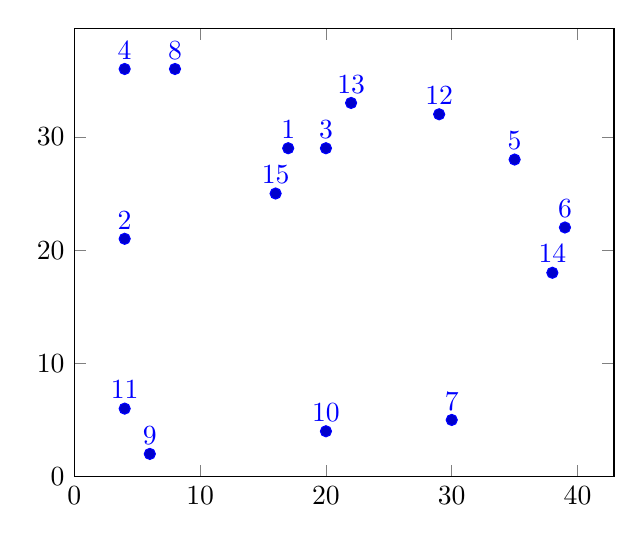
\begin{tikzpicture}
\begin{axis}[ymin = 0, xmin = 0]
  \addplot+[nodes near coords,only marks,
    point meta=explicit symbolic] 
  coordinates {
(17, 29) [1] 
(4, 21) [2] 
(20, 29) [3] 
(4, 36) [4] 
(35, 28) [5] 
(39, 22) [6] 
(30, 5) [7] 
(8, 36) [8] 
(6, 2) [9] 
(20, 4) [10]
(4, 6) [11]
(29, 32) [12]
(22, 33) [13]
(38, 18) [14]
(16, 25) [15]
  };
\end{axis}
\end{tikzpicture}
\end{center}


\newpage

\textbf{4b. Solution:}
\\
\\
\\
\textbf{VP Tree implementation - aka. Ball Positioning Tree}
\\
\\
\\
\\
VP Tree: Given the following VP tree, query point (25,4) with \epsilon = 11

The Euclidean distance formula for calculating distance between two co-ordinates (x1,y1) and (x2,y2) are


\[ d(p,q) = \sqrt{(x2-x1)^2+{(y2-y1)^2}} \]

We have to define if we want to go through the left sub-tree or right sub-tree.
Formula for calculating the left sub-tree is 
\[ {max(d(p,q)-r,0) \le \epsilon } \]

Formula for calculating the right sub-tree is
\[ {max(r-(d(p,q),0)  \le \epsilon } \]

\\

\begin{itemize}
    \item Distance between Root node \textbf{7:(30,5) and Query point (25,4)} with r = 26.01 and \epsilon = 11

\[ d(p,q) = \sqrt{(25-30)^2+{(4-5)^2}} = 5.09 \le 11 \quad \textbf{Add the node to tree} \] 
    Verifying if we should go through left sub-tree
    \[d(7,q)-r = 5.09-26.01 = -20.91 \]
    \[ {max(d(p,q)-r,0) \le \epsilon = {max(d(7,q)-r,0) = max(-20.91,0)} \le 11 \quad \textbf{Go through left sub-tree} \]
    
    Verifying if we should go through right sub-tree
     \[r-d(7,q) = 26.01-5.09 = 20.92 \]
    \[ {max(r-(d(p,q),0)  \le \epsilon } = {max(,0) = max(20.92,0)} \nleq 11 \quad  \textbf{Prune right sub-tree}\] 

    \textbf{Now we only consider the co-ordinates of the left sub-tree for the query point as we have pruned the right sub-tree}
\\
    
    \item Distance between \textbf{14: (38,18) and Query point (25,4)} with r = 21.95 and \epsilon = 11


    \[ d(14,q)= 19.10 \nleq 11 \quad \textbf{don't add node } \]

    Verify left sub-tree \[ max(-2.84,0) = 0 \le 11 \quad \textbf{ traverse through the left sub-tree}\]
    Verify right sub-tree \[ max(2.85,0) = 2,85 \le 11 \quad \textbf{ traverse through the right sub-tree}\]

    \item Distance between \textbf{6: (39,22) and Query point (25,4)} with r = 13.73 and \epsilon = 11

     \[ d(6,q)= 22.80 \nleq 11 \quad \textbf{don't add node } \]
     
    Verify left sub-tree \[ max(9.52,0) = 9.52 \le 11 \quad \textbf{ traverse through the left sub-tree}\]
    Verify right sub-tree \[ max(-9.07,0) = 0 \le 11 \quad \textbf{ traverse through the right sub-tree}\]

\newpage

    \item Distance between \textbf{15: (16,25) and Query point (25,4)} with r = 23.23 and \epsilon = 11

     \[ d(15,q)= 22.84 \nleq 11 \quad \textbf{don't add node } \]
     
    Verify left sub-tree \[ max(0.89,0) = 0 \le 11 \quad \textbf{ traverse through the left sub-tree}\]
    Verify right sub-tree \[ max(0.39,0) = 0 \le 11 \quad \textbf{ traverse through the right sub-tree}\]

    \item Distance between \textbf{5: (35,28) and Query point (25,4)} \epsilon = 11

     \[ d(5,q)= 26 \nleq 11 \quad \textbf{don't add node } \]

     \item Distance between \textbf{3: (20,29) and Query point (25,4)} \epsilon = 11

     \[ d(3,q)= 25.49 \nleq 11 \quad \textbf{don't add node } \]

     \item Distance between \textbf{10: (20,4) and Query point (25,4)} \epsilon = 11

     \[ d(10,q)= 5 \leq 11 \quad \textbf{ add node } \]

      \item Distance between \textbf{9: (6,2) and Query point (25,4)} \epsilon = 11

     \[ d(6,q)= 19.10 \nleq 11 \quad \textbf{don't add node } \]


     Hence \textbf{7 and 10 } nodes would be added to the result.




    
\end{itemize}
    
    



\end{document}


